% ============================================================
% FIFA World Cup 2026 — Importation Risk
% Collaborator presentation — LaTeX Beamer
% ============================================================
\documentclass[aspectratio=169, 11pt]{beamer}

% --- Theme ---------------------------------------------------
\usetheme{Madrid}
\usecolortheme{beaver}           % dark red headers, clean body
\setbeamertemplate{navigation symbols}{}   % remove nav clutter
\setbeamerfont{frametitle}{size=\large, series=\bfseries}

% --- Packages ------------------------------------------------
\usepackage{amsmath, amssymb}
\usepackage{booktabs}
\usepackage{array}
\usepackage{graphicx}
\usepackage{xcolor}
\usepackage{hyperref}
\usepackage{natbib}
\usepackage{tikz}
\usetikzlibrary{arrows.meta, positioning, shapes.geometric}

% --- Colours -------------------------------------------------
\definecolor{wcred}{RGB}{190, 30, 45}
\definecolor{wcblue}{RGB}{0, 64, 140}
\definecolor{wcgray}{RGB}{100, 100, 100}
\definecolor{baseline}{RGB}{67, 147, 195}
\definecolor{wcadj}{RGB}{214, 96, 77}
\definecolor{sched}{RGB}{116, 196, 118}

% --- Metadata ------------------------------------------------
\title[WC 2026 Importation Risk]{%
  Estimating Infectious Disease Importation Risk\\
  during the 2026 FIFA World Cup}
\author{Jose Herrera-Diestra}
\institute{Tarleton State University}
\date{May 2026}

% ============================================================
\begin{document}
% ============================================================

% --- Title slide --------------------------------------------
\begin{frame}
  \titlepage
\end{frame}

% --- Outline ------------------------------------------------
\begin{frame}{Outline}
  \tableofcontents[hideallsubsections]
\end{frame}

% ============================================================
\section{Context and question}
% ============================================================

\begin{frame}{The 2026 FIFA World Cup}
  \begin{columns}[T]
    \begin{column}{0.55\textwidth}
      \textbf{Key facts}
      \begin{itemize}
        \item \textbf{48 nations} — largest World Cup in history
        \item \textbf{3 co-host countries}: USA, Mexico, Canada
        \item \textbf{16 venues} across 11 US cities, 2 Canadian,
              3 Mexican
        \item Matches from \textbf{June 11 – July 19, 2026}
        \item Expected \textbf{$\sim$85 million} international
              arrivals to the US in June 2026 alone (NTTO forecast)
        \item Tickets sold to fans from all 48 qualified nations
      \end{itemize}
    \end{column}
    \begin{column}{0.42\textwidth}
      \vspace{0.5em}
      \begin{block}{Why does this matter?}
        Mass gathering events accelerate the \textbf{importation}
        of infectious diseases into host cities.
        Early quantification helps public health authorities
        prioritise \textbf{surveillance} and
        \textbf{preparedness} by venue.
      \end{block}
    \end{column}
  \end{columns}
\end{frame}

% ------------------------------------------------------------
\begin{frame}{Venue cities — 16 stadiums across North America}
  \begin{center}
    \includegraphics[width=\textwidth, height=0.7\textheight, keepaspectratio]%
      {../Figures/wc2026_venue_map.png}
  \end{center}
  \vspace{-0.5em}
  {\footnotesize \textbf{Blue}: 11 US venues \quad
   \textbf{Red}: 2 Canadian venues \quad
   \textbf{Green}: 3 Mexican venues. \quad
   Suburb names mapped to metro areas (e.g.\ East Rutherford $\to$ New York).}
\end{frame}

% ------------------------------------------------------------
\begin{frame}{Scientific question}
  \begin{center}
    \large
    \textit{What is the probability that at least one case of
    dengue, malaria, measles, or pertussis is \textbf{imported}
    into each WC host city during June 2026 — and which
    source countries drive that risk?}
  \end{center}

  \vspace{1em}
  \begin{columns}[T]
    \begin{column}{0.48\textwidth}
      \textbf{Four diseases studied}
      \begin{itemize}
        \item \textbf{Dengue} — endemic in Latin America, SE Asia,
              Africa; strongly seasonal
        \item \textbf{Malaria} — sub-Saharan Africa, SE Asia,
              Middle East
        \item \textbf{Measles} — resurgent globally; under-vaccinated
              pockets
        \item \textbf{Pertussis} — globally endemic; early
              infectious phase easily missed
      \end{itemize}
    \end{column}
    \begin{column}{0.48\textwidth}
      \textbf{Three nested models}
      \begin{enumerate}
        \item \textcolor{baseline}{\textbf{Baseline}} — COR June 2024
              $\times$ T-100 routing, no WC adjustment
        \item \textcolor{wcadj}{\textbf{WC-adjusted}} — 2026 country-level
              travel surge
        \item \textcolor{sched}{\textbf{Schedule-driven}} — fan routing
              by match schedule
      \end{enumerate}
    \end{column}
  \end{columns}
\end{frame}

% ============================================================
\section{Methods}
% ============================================================

\begin{frame}{The Poisson importation framework}
  We model disease importation as a \textbf{Poisson process}.

  \bigskip
  If $\Lambda_{v,d}$ is the \textit{expected} number of imported cases
  of disease $d$ arriving in city $v$, the probability of at least one
  importation is:

  \begin{equation}
    \boxed{P(X_{v,d} \geq 1) = 1 - e^{-\Lambda_{v,d}}}
    \tag{Poisson}
  \end{equation}

  where $\Lambda_{v,d} = \displaystyle\sum_{c} \lambda_{c,v,d}$
  sums over all source countries $c$.

  \bigskip
  Each country-level contribution has the same structure across all
  three models:
  \[
    \lambda_{c,v,d}
    = \underbrace{N_{c,v}}_{\text{arrivals}}
    \;\times\;
    \underbrace{I_{c,d}}_{\substack{\text{per-traveller}\\\text{infection prob.}}}
    \;\times\;
    \underbrace{p_d}_{\substack{\text{travel while}\\\text{infectious}}}
  \]
\end{frame}

% ------------------------------------------------------------
\begin{frame}{Disease-specific parameters}
  \begin{center}
  \footnotesize
  \begin{tabular}{lcccl}
    \toprule
    \textbf{Disease}
      & \textbf{$\rho_d$ range}
      & \textbf{$\rho_d$ (used)}
      & \textbf{$p_d$}
      & \textbf{Rationale for $p_d$} \\
    \midrule
    Dengue
      & 0.06--0.26 & \textbf{0.10} & 0.50
      & Mild viremia; $\sim$40\% viremic at arrival \\
    Malaria
      & 0.10--0.35 & \textbf{0.20} & 0.30
      & Severe illness; most febrile after return \\
    Measles
      & 0.10--0.60 & \textbf{0.60} & 0.05
      & Prostrating; only short pre-rash window \\
    Pertussis
      & 0.01--0.10 & \textbf{0.10} & 0.70
      & Catarrhal stage $\approx$ common cold; unrecognised \\
    \bottomrule
  \end{tabular}
  \end{center}

  \smallskip
  {\footnotesize
  $\rho_d$ range from: Bhatt et al.\ 2013 (dengue);
  WHO WMR 2024 (malaria); Simons et al.\ 2012 (measles);
  McLaughlin et al.\ 2016 (pertussis).}

  \smallskip
  $\rho_d$ — \textbf{reporting adjustment} $\cdot$
  $p_d$ — \textbf{travel-while-infectious probability} $\cdot$
  $I_{c,d} = \rho_d \cdot C_{c,d} / P_c$
\end{frame}

% ------------------------------------------------------------
\begin{frame}{Data sources}
  \begin{columns}[T]
    \begin{column}{0.48\textwidth}
      \textbf{Travel data}
      \begin{itemize}
        \item \textbf{BTS T-100 International Segment}: nonstop
              flight segments at individual US airports (June
              2023--2025) — country-level routing fractions for all
              \textbf{11 US venue cities}; used in all 3 models
        \item \textbf{COR I-94 data} (CBP): monthly arrivals by
              country of residence — June 2024 used as baseline
              (no WC growth for Model 1)
        \item \textbf{NTTO 2026 Forecast} (trade.gov): official
              2026 projections for 12 top source markets
      \end{itemize}
    \end{column}
    \begin{column}{0.48\textwidth}
      \textbf{Disease data}
      \begin{itemize}
        \item \textbf{Dengue}: WHO Global Dengue Surveillance
              (monthly, accessed Dec 2025)
        \item \textbf{Malaria}: WHO Global Malaria Programme
              National Unit Data (2024 annual)
        \item \textbf{Measles}: WHO Immunization Data portal
              (annual, accessed Sep 2025)
        \item \textbf{Pertussis}: WHO Immunization Data portal
              (annual, accessed Dec 2025)
      \end{itemize}
      \vspace{0.5em}
      \textbf{Match schedule}: 69 games (group stage) across
      16 venues from FIFA event records
    \end{column}
  \end{columns}
\end{frame}

% ------------------------------------------------------------
\begin{frame}{Three-model hierarchy}
  \begin{center}
  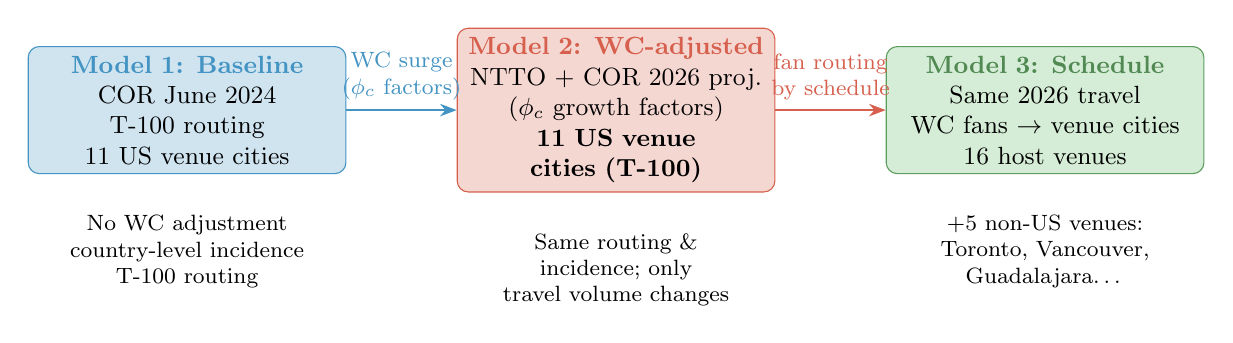
\begin{tikzpicture}[
    node distance = 1.6cm,
    box/.style = {rectangle, rounded corners, draw, text width=3.8cm,
                  minimum height=1.4cm, align=center, font=\small},
    arrow/.style = {-{Stealth[length=6pt]}, thick}
  ]
    \node[box, fill=baseline!25, draw=baseline] (m1)
      {\textcolor{baseline}{\textbf{Model 1: Baseline}}\\
       COR June 2024\\T-100 routing\\
       11 US venue cities};

    \node[box, fill=wcadj!25, draw=wcadj, right=1.4cm of m1] (m2)
      {\textcolor{wcadj}{\textbf{Model 2: WC-adjusted}}\\
       NTTO + COR 2026 proj.\\($\phi_c$ growth factors)\\
       \textbf{11 US venue cities (T-100)}};

    \node[box, fill=sched!30, draw=sched!80!black, right=1.4cm of m2] (m3)
      {\textcolor{sched!70!black}{\textbf{Model 3: Schedule}}\\
       Same 2026 travel\\WC fans $\to$ venue cities\\
       16 host venues};

    \draw[arrow, color=baseline] (m1) --
      node[above, font=\footnotesize, align=center, text width=2.2cm]
        {WC surge\\($\phi_c$ factors)} (m2);
    \draw[arrow, color=wcadj] (m2) --
      node[above, font=\footnotesize, align=center, text width=2cm]
        {fan routing\\by schedule} (m3);

    \node[below=0.4cm of m1, font=\footnotesize, text width=3.8cm, align=center]
      {No WC adjustment\\country-level incidence\\T-100 routing};
    \node[below=0.4cm of m2, font=\footnotesize, text width=3.8cm, align=center]
      {Same routing \&\\incidence; only\\travel volume changes};
    \node[below=0.4cm of m3, font=\footnotesize, text width=3.8cm, align=center]
      {+5 non-US venues:\\Toronto, Vancouver,\\Guadalajara\ldots};
  \end{tikzpicture}
  \end{center}

  \smallskip
  \textbf{M1 $\to$ M2}: isolates the WC travel surge ($\phi_c$
  growth factors applied to COR 2024 base volumes).\\
  \textbf{M2 $\to$ M3}: isolates schedule-based fan routing; adds
  5 non-US venues.
\end{frame}

% ------------------------------------------------------------
\begin{frame}{Model 1 — Baseline: equations}
  \textbf{Why T-100 routing for the baseline?}
  T-100 covers all \textbf{11 US venue cities} at country level,
  making it the only source that provides a consistent spatial grid
  across all three models --- so M1 $\to$ M2 isolates travel volume
  only.

  \medskip
  \textbf{Baseline arrivals} (COR June 2024, no WC growth):
  \begin{equation}
    N_{c,v}^{\text{baseline}} = N_{c,\text{Jun 2024}}^{\text{COR}}
      \cdot f_{c,v}^{\text{T100}}
    \tag{baseline arrivals}
  \end{equation}

  \textbf{Country-level incidence} (shared across all 3 models):
  \begin{equation}
    I_{c,d} = \rho_d \cdot \frac{C_{c,d}}{P_c}
    \tag{incidence}
  \end{equation}

  \textbf{Importation intensity}:
  \begin{equation}
    \lambda_{c,v,d} = N_{c,v}^{\text{baseline}} \cdot I_{c,d} \cdot p_d
    \qquad
    \Lambda_{v,d} = \sum_{c} \lambda_{c,v,d}
    \tag{baseline $\lambda$}
  \end{equation}
\end{frame}

% ------------------------------------------------------------
\begin{frame}{Model 2 — WC-adjusted: travel volume construction}
  \textbf{Tiered approach} to 2026 travel volume:

  \begin{block}{Tier 1 — NTTO top-12 markets (Australia, Brazil, Canada,
    China, France, Germany, India, Italy, Japan, Mexico, South Korea, UK)}
    Growth factor $\phi_c = V_{c,2026}/V_{c,2024}$ from official
    NTTO Forecast Report. Already includes WC effect — \textit{do not}
    add WC visitors on top.
  \end{block}

  \begin{block}{Remaining countries (COR I-94, June 2024)}
    \begin{itemize}
      \item WC-qualified: $\phi_{\text{WC}} = 85{,}017/72{,}390
            = \mathbf{1.174}$ (aggregate NTTO WC uplift)
      \item Non-qualified: $\phi_{\text{base}} = \mathbf{1.077}$
            — data-driven from COR + T-100 June 2023--2025\\
            {\footnotesize
             $\bar{g} = \sqrt{N_{2024}/N_{2023}\;\cdot\;N_{2025}/N_{2024}}$,\;
             $\phi_{\text{base}} = \bar{g}^{\,2}$;\;
             COR: 1.062 \quad T-100: 1.092 \quad avg: \textbf{1.077}}
    \end{itemize}
  \end{block}

  \vspace{-6pt}
  \[
    N_{c,\,\text{Jun 2026}} = N_{c,\,\text{Jun 2024}}^{\text{COR}} \cdot \phi_c
    \quad
    N_{c,v}^{2026} = N_{c,\,\text{Jun 2026}} \cdot f_{c,v}^{\text{T100}}
  \]
  {\footnotesize $f_{c,v}^{\text{T100}}$: T-100 routing fraction (mean June 2023--2025),
  same in all three models, covering \textbf{all 11 US venue cities}.}
\end{frame}

% ------------------------------------------------------------
\begin{frame}{Model 2 — WC-adjusted: incidence and $\lambda$}
  \textbf{Country-level incidence} (more precise than regional):
  \begin{equation}
    I_{c,d} = \rho_d \cdot \frac{C_{c,d}}{P_c}
    \tag{country incidence}
  \end{equation}

  \textbf{Importation intensity}:
  \begin{equation}
    \lambda_{c,v,d} = N_{c,v}^{2026} \cdot I_{c,d} \cdot p_d
    \qquad
    \Lambda_{v,d} = \sum_{c}\, \lambda_{c,v,d}
    \tag{WC-adj $\lambda$}
  \end{equation}

  \bigskip
  \textbf{What changes from Model 1:}
  \begin{itemize}
    \item Travel volume reflects the WC surge ($\phi_c$ growth factors
          applied to COR June 2024 base volumes)
    \item Routing fractions, city coverage, disease incidence,
          $\rho_d$ and $p_d$ are \textbf{unchanged} from Model 1
    \item[$\Rightarrow$] M1 $\to$ M2 isolates the WC travel surge alone
  \end{itemize}
\end{frame}

% ------------------------------------------------------------
\begin{frame}{Model 3 — Schedule-driven: the core idea}
  \begin{columns}[T]
    \begin{column}{0.55\textwidth}
      \textbf{Problem with Models 1 \& 2}\\
      T-100 routing fractions reflect habitual tourist flows; WC fans
      travel to the specific cities where their team plays.

      \medskip
      \textbf{Reality}: fans from Brazil go to \textit{Houston}
      (where Brazil plays), not to Boston or Philadelphia.

      \medskip
      \textbf{Solution}: separate the WC-specific travel increment
      from background tourism, and route fans using the match schedule.
    \end{column}
    \begin{column}{0.42\textwidth}
      \begin{alertblock}{Travel decomposition}
        \[
          N_c^{\text{WC}} = N_{c,24}^{\text{COR}}
            \cdot \max\!\bigl(0,\; \phi_c - \phi_{\text{base}}\bigr)
        \]
        \[
          N_c^{\text{bg}} = N_{c,\text{Jun 2026}} - N_c^{\text{WC}}
        \]
        For WC-qualified countries:\\
        WC increment $\approx 8.3\%$ of projected arrivals
        \[
          \frac{1.174 - 1.077}{1.174} \approx 0.083
        \]
      \end{alertblock}
    \end{column}
  \end{columns}
\end{frame}

% ------------------------------------------------------------
\begin{frame}{Model 3 — Schedule-driven: routing equations}
  \textbf{Schedule-based WC fan routing fraction}:
  \begin{equation}
    \omega_{c,v} = \frac{g_{c,v}}{G_c}
    \tag{schedule routing}
  \end{equation}
  $g_{c,v}$ = games played by country $c$'s team at venue city $v$;
  $G_c$ = total known group-stage games.

  \medskip
  \textbf{Arrival matrices}:
  \[
    N_{c,v}^{\text{WC}} = N_c^{\text{WC}} \cdot \omega_{c,v}
    \qquad\text{(WC fans $\to$ venue cities)}
  \]
  \[
    N_{c,v}^{\text{bg}} = N_c^{\text{bg}} \cdot f_{c,v}^{\text{T100}}
    \qquad\text{(background $\to$ all 11 US cities via T-100)}
  \]

  \textbf{Combined importation intensity for venue city $v$}:
  \begin{equation}
    \Lambda_{v,d} =
      \underbrace{%
        \sum_{c \in \mathcal{Q}} N_{c,v}^{\text{WC}} \cdot I_{c,d} \cdot p_d
      }_{\text{WC fans}}
      +
      \underbrace{%
        \sum_{c} N_{c,v}^{\text{bg}} \cdot I_{c,d} \cdot p_d
      }_{\text{background}}
    \tag{schedule $\lambda$}
  \end{equation}
\end{frame}

% ------------------------------------------------------------
\begin{frame}{Model 3 — Venue coverage}
  \begin{columns}[T]
    \begin{column}{0.52\textwidth}
      \footnotesize
      \begin{tabular}{lll}
        \toprule
        \textbf{City} & \textbf{Country} & \textbf{T-100 bg?} \\
        \midrule
        New York       & USA    & \textcolor{wcblue}{Yes} \\
        Dallas         & USA    & \textcolor{wcblue}{Yes} \\
        Houston        & USA    & \textcolor{wcblue}{Yes} \\
        Philadelphia   & USA    & \textcolor{wcblue}{Yes} \\
        Boston         & USA    & \textcolor{wcblue}{Yes} \\
        Los Angeles    & USA    & \textcolor{wcblue}{Yes} \\
        Atlanta        & USA    & \textcolor{wcblue}{Yes} \\
        Kansas City    & USA    & \textcolor{wcblue}{Yes*} \\
        Miami          & USA    & \textcolor{wcblue}{Yes} \\
        San Francisco  & USA    & \textcolor{wcblue}{Yes} \\
        Seattle        & USA    & \textcolor{wcblue}{Yes} \\
        Vancouver      & Canada & No \\
        Toronto        & Canada & No \\
        Mexico City    & Mexico & No \\
        Monterrey      & Mexico & No \\
        Guadalajara    & Mexico & No \\
        \bottomrule
      \end{tabular}
      {\tiny * Near-zero fractions; mainly WC-fan stream}
    \end{column}
    \begin{column}{0.45\textwidth}
      \small
      \begin{block}{Key insight}
        \textcolor{baseline}{\textbf{11 US cities}}: both WC-fan
        and background streams contribute (T-100 covers all).
      \end{block}
      \begin{block}{}
        \textcolor{wcgray}{\textbf{5 non-US venues}}: only the
        WC-fan stream contributes.\\
        \textit{No T-100 data for Canada/Mexico cities.}
      \end{block}
      \smallskip
      \textbf{England + Scotland issue:}\\
      Both map to ``United Kingdom'' in COR data. Routing fractions
      sum to 1 — no double-counting.
    \end{column}
  \end{columns}
\end{frame}

% ============================================================
\section{Results}
% ============================================================

\begin{frame}{Model 1 — Baseline results}
  \begin{center}
    \includegraphics[width=\textwidth, height=0.68\textheight, keepaspectratio]%
      {../Figures/estimated_importations.png}
  \end{center}
  \vspace{-0.3em}
  {\footnotesize Numbers above bars = $P(\geq 1\,\text{importation})$;
  bar height = expected importation intensity $\lambda$.}
\end{frame}

% ------------------------------------------------------------
\begin{frame}{Model 2 — WC-adjusted results}
  \begin{center}
    \includegraphics[width=\textwidth, height=0.68\textheight, keepaspectratio]%
      {../Figures/estimated_importations_wc_adjusted.png}
  \end{center}
  \vspace{-0.3em}
  {\footnotesize All 11 US venue cities (same as Model 1); travel
  volumes now reflect June 2026 projections ($\phi_c$ growth factors).}
\end{frame}

% ------------------------------------------------------------
\begin{frame}{Model 3 — Schedule-driven results}
  \begin{center}
    \includegraphics[width=\textwidth, height=0.68\textheight, keepaspectratio]%
      {../Figures/estimated_importations_schedule_driven.png}
  \end{center}
  \vspace{-0.3em}
  {\footnotesize Up to 16 venue cities visible; WC fans are routed to
  where their team plays; background travelers use T-100 routing.}
\end{frame}

% ------------------------------------------------------------
\begin{frame}{Three-model comparison — importation probability}
  \begin{center}
    \includegraphics[width=\textwidth, height=0.68\textheight, keepaspectratio]%
      {../Figures/model_comparison_probability.png}
  \end{center}
  \vspace{-0.3em}
  {\footnotesize \textcolor{baseline}{$\blacksquare$ Baseline} \quad
   \textcolor{wcadj}{$\blacksquare$ WC-adjusted} \quad
   \textcolor{sched}{$\blacksquare$ Schedule-driven}. \quad
   $P(\geq 1)$ saturates to 1 for high-risk cities — see next slide
   for the linear-scale $\lambda$ comparison.}
\end{frame}

% ------------------------------------------------------------
\begin{frame}{Three-model comparison — importation intensity ($\lambda$)}
  \begin{center}
    \includegraphics[width=\textwidth, height=0.68\textheight, keepaspectratio]%
      {../Figures/model_comparison_intensity.png}
  \end{center}
  \vspace{-0.3em}
  {\footnotesize $\lambda$ stays linear even when $P(\geq 1) \to 1$,
   revealing relative risk more clearly than the probability scale.}
\end{frame}

% ============================================================
\section{Country contributions}
% ============================================================

\begin{frame}{Which countries drive importation risk?}
  \begin{center}
    \includegraphics[width=\textwidth, height=0.68\textheight, keepaspectratio]%
      {../Figures/country_importation_ranking.png}
  \end{center}
  \vspace{-0.3em}
  {\footnotesize Top 15 source countries by total expected importations
  (schedule-driven model, summed across all destination cities).}
\end{frame}

% ------------------------------------------------------------
\begin{frame}{WC fans vs.\ background tourists — dengue}
  \begin{center}
    \includegraphics[width=\textwidth, height=0.68\textheight, keepaspectratio]%
      {../Figures/stream_breakdown_dengue.png}
  \end{center}
  \vspace{-0.3em}
  {\footnotesize
    \textcolor{wcadj}{$\blacksquare$ WC fans} \quad
    \textcolor{baseline}{$\blacksquare$ Background}.
    Countries with WC teams show a non-zero WC-fan component;
    non-qualified countries contribute only through background travel.}
\end{frame}

% ------------------------------------------------------------
\begin{frame}{Country $\times$ city importation matrix — dengue}
  \begin{center}
    \includegraphics[width=\textwidth, height=0.68\textheight, keepaspectratio]%
      {../Figures/heatmap_dengue.png}
  \end{center}
  \vspace{-0.3em}
  {\footnotesize Colour = expected dengue importations $\lambda_{c,v}$.
  WC-qualified countries show concentration in specific match venues;
  non-qualified countries show diffuse contributions via T-100 routing.}
\end{frame}

% ============================================================
\section{Key findings \& Limitations}
% ============================================================

\begin{frame}{Key findings}
  \begin{enumerate}
    \item \textbf{Dengue dominates} importation intensity across all
          three models and all destination cities, driven by high
          incidence in Latin America and SE Asia.
    \item \textbf{The WC travel surge} (Model 1 $\to$ 2) increases
          estimated importation intensity for qualified nations but
          city rankings remain broadly stable.
    \item \textbf{Schedule-driven routing} (Model 2 $\to$ 3) reveals
          concentration of risk at specific match venues (e.g.,
          Houston for Brazil games) and adds the 5 non-US venues
          (Toronto, Vancouver, Guadalajara, Mexico City, Monterrey).
    \item \textbf{Background travel} dominates the total importation
          burden for most diseases; the WC-fan increment is $\approx
          8.3\%$ of projected arrivals for qualified countries.
    \item \textbf{A small number of high-incidence countries} (Brazil,
          Colombia, and others by disease) account for a
          disproportionate share of city-level risk.
  \end{enumerate}
\end{frame}

% ------------------------------------------------------------
\begin{frame}{Limitations}
  \small
  \begin{columns}[T]
    \begin{column}{0.48\textwidth}
      \textbf{Parameter uncertainty}
      \begin{itemize}
        \item $\rho_d$ and $p_d$ are central estimates — no strong
              empirical constraint for mass sporting events
        \item Sensitivity analysis ($\pm50\%$) recommended before
              policy communication
      \end{itemize}
      \vspace{2pt}
      \textbf{Travel data coverage}
      \begin{itemize}
        \item T-100 covers all 11 US venue cities across all models
        \item 5 non-US venues receive only WC-fan stream —
              background risk underestimated there
        \item T-100 covers nonstop segments only; connecting
              passengers appear at entry city
      \end{itemize}
    \end{column}
    \begin{column}{0.48\textwidth}
      \textbf{Model scope}
      \begin{itemize}
        \item Importation only — no secondary transmission
        \item Knockout-round games excluded (TBD opponents)
        \item Fan routing assumes proportional allocation by
              games; actual behaviour may differ
      \end{itemize}
      \vspace{2pt}
      \textbf{Data recency}
      \begin{itemize}
        \item Disease data through late 2025; current outbreak
              situations may differ
        \item NTTO projections pre-date the event; actual
              arrival volumes will vary
      \end{itemize}
    \end{column}
  \end{columns}
\end{frame}

% ------------------------------------------------------------
\begin{frame}{Data that would most improve the model}
  \begin{columns}[T]
    \begin{column}{0.33\textwidth}
      \textbf{Travel volume}
      \begin{itemize}\small
        \item \textbf{Flight bookings} (OAG, Amadeus, IATA PaxIS) —
              direct country-to-city routing for June 2026
        \item \textbf{FIFA ticket sales} by country — most direct
              measure of WC fan travel; replaces NTTO
              decomposition
        \item \textbf{Previous WC entry records} (Brazil 2014,
              Russia 2018, Qatar 2022) — empirical validation
              of fan routing
      \end{itemize}
    \end{column}
    \begin{column}{0.33\textwidth}
      \textbf{Disease burden}
      \begin{itemize}\small
        \item \textbf{Real-time surveillance} (ProMED, WHO DON,
              ECDC CDTR) — catch outbreaks after the 2025
              data freeze
        \item \textbf{Age-stratified incidence} — travelers skew
              working-age; refines $I_{c,d}$
        \item \textbf{Vaccination coverage} (WHO/UNICEF) — adjust
              effective measles/pertussis incidence for
              traveler immunity
      \end{itemize}
    \end{column}
    \begin{column}{0.33\textwidth}
      \textbf{Local transmission}
      \begin{itemize}\small
        \item \textbf{\textit{Ae.~aegypti} surveillance} (CDC
              ArboNET) — extend to local dengue outbreak
              probability
        \item \textbf{Hospital capacity} (AHA survey) —
              contextualise risk for health-system
              pre-positioning
        \item \textbf{Mobility data} (Meta, Google) —
              validate schedule-based fan routing
              empirically
      \end{itemize}
    \end{column}
  \end{columns}
\end{frame}

% ------------------------------------------------------------
\begin{frame}{WC fans vs.\ background — malaria, measles, pertussis}
  \begin{center}
    \includegraphics[width=\textwidth, height=0.68\textheight, keepaspectratio]%
      {../Figures/stream_breakdown_panel.png}
  \end{center}
  \vspace{-0.3em}
  {\footnotesize All four diseases. \textcolor{wcadj}{$\blacksquare$ WC fans} \quad
   \textcolor{baseline}{$\blacksquare$ Background}.
   Background dominates total importation burden for most countries;
   WC-fan increment $\approx 8.3\%$ of projected arrivals for qualified nations.}
\end{frame}

% ------------------------------------------------------------
\begin{frame}{Country $\times$ city matrix — malaria}
  \begin{center}
    \includegraphics[width=\textwidth, height=0.68\textheight, keepaspectratio]%
      {../Figures/heatmap_malaria.png}
  \end{center}
  \vspace{-0.3em}
  {\footnotesize Risk concentrated in West and Central African source countries
  at their specific match venues.}
\end{frame}

% ------------------------------------------------------------
\begin{frame}{Country $\times$ city matrix — measles \& pertussis}
  \begin{columns}[T]
    \begin{column}{0.5\textwidth}
      \includegraphics[width=\textwidth, height=0.55\textheight, keepaspectratio]%
        {../Figures/heatmap_measles.png}
      {\tiny Measles: low absolute intensities due to $p = 0.05$}
    \end{column}
    \begin{column}{0.5\textwidth}
      \includegraphics[width=\textwidth, height=0.55\textheight, keepaspectratio]%
        {../Figures/heatmap_pertussis.png}
      {\tiny Pertussis: broad geographic spread; $p = 0.70$}
    \end{column}
  \end{columns}
\end{frame}

% ============================================================
\section{Sensitivity analysis}
% ============================================================

\begin{frame}{Sensitivity analysis — absolute $\lambda$}
  \begin{center}
    \includegraphics[width=\textwidth, height=0.68\textheight, keepaspectratio]%
      {../Figures/sensitivity_analysis_lambda.png}
  \end{center}
  \vspace{-0.3em}
  {\footnotesize $\rho_d$ and $p_d$ each varied $\times$0.50 -- $\times$1.50
   independently. $\Lambda$ is strictly linear in both parameters.}
\end{frame}

% ------------------------------------------------------------
\begin{frame}{Sensitivity analysis — relative $P(\geq 1)$}
  \begin{center}
    \includegraphics[width=\textwidth, height=0.68\textheight, keepaspectratio]%
      {../Figures/sensitivity_analysis_relative.png}
  \end{center}
  \vspace{-0.3em}
  {\footnotesize $P(\geq 1)_{\text{perturbed}} / P(\geq 1)_{\text{central}}$.
   High-$\Lambda$ cities (near-certain importation) are \textbf{insensitive}
   to $\pm$50\% parameter errors; mid-range cities show the largest relative
   shifts — city rankings are \textbf{robust} at the top.}
\end{frame}

% ------------------------------------------------------------
\begin{frame}{Sensitivity analysis — absolute $\Delta P(\geq 1)$}
  \begin{center}
    \includegraphics[width=\textwidth, height=0.68\textheight, keepaspectratio]%
      {../Figures/sensitivity_analysis_delta_prob.png}
  \end{center}
  \vspace{-0.3em}
  {\footnotesize Absolute probability shift $\Delta P = P_{\text{perturbed}} -
   P_{\text{central}}$. Peak uncertainty falls on \textbf{mid-range} cities,
   not highest-risk destinations already near certainty.}
\end{frame}

\begin{frame}{Next steps}
  \begin{enumerate}
    \item \textbf{Airport-level allocation} — distribute city-level
          importation risk across individual US airports using BTS
          enplanement data and spatial join to counties (code
          already in supplementary file)

    \item \textbf{Incorporate knockout rounds} — as the WC bracket
          becomes known, update the schedule-driven model with
          resolved match assignments

    \item \textbf{Real-time surveillance linkage} — compare model
          predictions against actual case notifications from CDC
          and partner health agencies during the tournament

    \item \textbf{Expand disease scope} — cholera, mpox, and
          influenza are under consideration for a follow-up analysis

    \item \textbf{Canadian and Mexican venue routing} — obtain
          Statistics Canada and SICT/IATA data to extend T-100-style
          routing fractions to non-US host cities
  \end{enumerate}
\end{frame}

% ------------------------------------------------------------
\begin{frame}[plain]
  \vfill
  \begin{center}
    {\Large\textbf{Thank you}}\\[1em]
    \texttt{jherreradiestra@tarleton.edu}\\[0.8em]
    {\small Code and data:}\\[0.2em]
    {\small\url{https://github.com/jdiestra1977/FIFA_worldCup_2026_risk}}
  \end{center}
  \vfill
\end{frame}

% ============================================================
\end{document}
